\section{Topic 1. Error Sources and Floating Point Numbers}
Many problems in science and engineering are described using continuous variables and then  modelled by differential equations.

\begin{table}[h]
\begin{tabularx}{\textwidth}{ll}
\toprule
\textbf{Fluid Mechanics}  & Laws of Motion             \\
\textbf{Electromagnetism} & Maxwell's Equations        \\
\textbf{Stock Pricing}    & Black-Scholes Equation     \\
\textbf{Machine Learning} & Neural Networks \\
\bottomrule \\
\end{tabularx}
\end{table}

\noindent Since computers have finite resources, we must approximate solutions to these problems in finite precision. This involves,

\begin{table}[h]
\begin{tabularx}{\textwidth}{ll}
\toprule
\textbf{Validation}  & - Accurate approximations of solutions \\
                     & - Efficiency in costs \\
                     & - Stability during computation \\
\textbf{Verification} & - Accurate models of real-world phenomenon \\
\bottomrule \\
\end{tabularx}
\end{table}

\begin{center}
       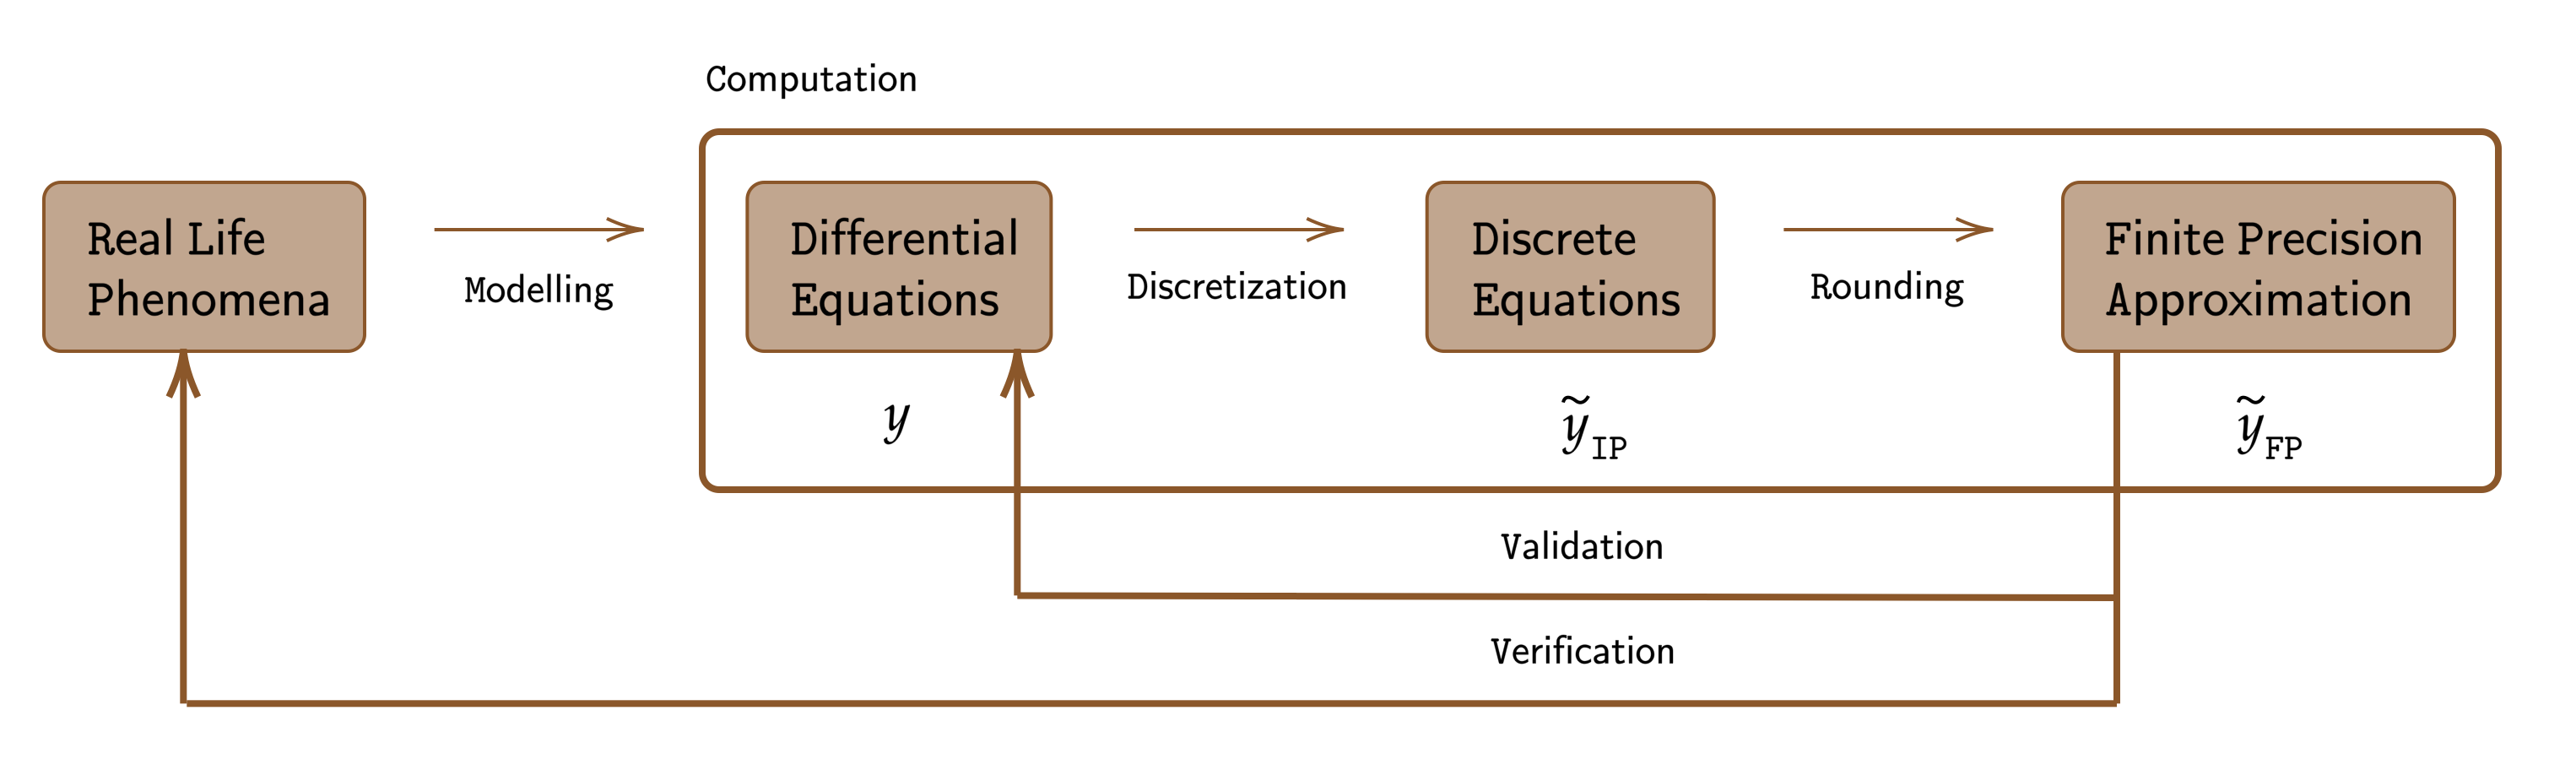
\includegraphics[width=\textwidth]{figures/fig-1.png}
\end{center}

\begin{marginfigure}
    We will use the following notation,
    \begin{align*}
        x &\quad\quad \text{Exact input value} \\
        \tilde{x} &\quad\quad \text{Approximate input value} \\
        f &\quad\quad \text{Exact output value} \\
        \fpa &\quad\quad \text{Finite-precision approximation}
    \end{align*}
\end{marginfigure}

\subsection{Rounding and Discretization}
\begin{defn}[Discretization Error]
    \sloppy The \textbf{discretization error} is an infinite-precision measurement of the difference between the exact output and the numerical output,
    \[\left|f(x)-\ipa(x)\right|\]
\end{defn}

\begin{defn}[Rounding Error]
   \sloppy The \textbf{rounding error} is an infinite-precision measurement of the difference between numerical outputs with infinite and finite precision,
   \[\left|\ipa(x)-\fpa(x)\right|\]
\end{defn}

\begin{rmk}
   Error sources from computation can be bounded by,
   \begin{align*}
    \text { Error } &:=|f(x)-\tilde{f}(\tilde{x})| \\
    & \leq \underbrace{|f(x)-f(\tilde{x})|}_{\text {Data Error }}+\underbrace{|f(\tilde{x})-\fpa(\tilde{x})|}_{\text {Computation Error }}
    \end{align*}
    Assuming no data error, i.e., $x = \tilde{x}$, we have, 
    \begin{align*}
        |f(\tilde{x})-\fpa(x)| &= |f(x)-\fpa(x)| \\
        &\leq \underbrace{\left|f(x)-\ipa(x)\right|}_{\text {Discretization Error }}+\underbrace{\left|\ipa(x)-\fpa(x)\right|}_{\text {Rounding Error }}
    \end{align*}
    as our bound on the computation error.
\end{rmk}

\begin{ex}{Computation Error}{label}
    Let $f(x) = \sin (x)$. We will approximate $f$ using,
    \begin{align*}
        &\ipa(x) = x \text{ in infinite precision} \\
        &\fpa(x) = x \text{ with the first four non-zero digits}
    \end{align*}
    
   What is the discretization and rounding error at $x = 1/9$?
   
    \LineBreak
    
    We begin with the following computations,
    \begin{align*}
        &f(1 / 9)=\sin (1 / 9) = 0.11088262851 \ldots \\
        &\ipa(1 / 9) = 1 / 9 = 0.11111111111 \ldots \\
        &\fpa(1 / 9) = 0.1111
    \end{align*}
    allowing us to conclude for the choice of $x = 1/9$ that,
    \begin{enumerate}
        \item The \textbf{discretization error} is defined by $\left|\sin(x)-\ipa(x)\right|$. So,
        \[\left|\sin(1/9) - 1/9\right| = 0.0002284826 \ldots \]
        \item The \textbf{rounding error} is defined by $\left|\ipa(x)-\fpa(x)\right|$. So,
        \[\left|1/9 - 0.1111\right| = 0.0000111111 \ldots \]
        \item The \textbf{computation error} is defined by $|f(x)-\fpa(x)|$. So,
        \begin{align*}
            \left|f(1 / 9)-\fpa(1 / 9)\right| &= 0.00021737149 \\
            &\leq 0.0002284826+0.0000111111 \\
            &= \text {Discretization Error} + \text {Rounding Error}
        \end{align*}
    \end{enumerate}
\end{ex}

\subsection{Measuring Error}
Consider a non-zero real number $a$ and its approximation $\tilde{a}$.

\begin{defn}[Absolute Error]
    \sloppy The \textbf{absolute error} is the difference between measured or inferred value $\tilde{x}$ and the actual value of $x$,
    \[|x-\tilde{x}|\]
\end{defn}

\begin{rmk}
    \sloppy The absolute error is inadequate due to the fact that it does not give any details regarding the importance of the error.
\end{rmk}

\begin{defn}[Relative Error]
    \sloppy The \textbf{relative error} is the ratio of the absolute error of the measurement to the actual value of $x$,
    \[\frac{1}{|x|} \cdot |x-\tilde{x}|\]
    The relative error is defined to be $1$ when $x = 0$.
\end{defn}

\begin{rmk}
    \sloppy This allows us to determine the magnitude of the absolute error in terms of the actual size of the measurement.
\end{rmk}

\begin{ex}{Absolute and Relative Error}{label}
    Let $f(x) = \sqrt{x}$. We will approximate $f$ using,
    \[\fpa(x) = \sqrt{x} \text{ with the first two non-zero digits}\]
    What is the absolute and relative error at $x = 2$?
    
    \LineBreak
    
    We begin with the following computations,
    \begin{align*}
    &f(2)=\sqrt{2}=1.41421356237 \ldots \\
    &\fpa(2)=1.4
    \end{align*}
    allowing us to conclude for the choice of $x = 2$ that,
    \begin{enumerate}
        \item The \textbf{absolute error} is defined by $|f(x) - \fpa(x)|$. So,
        \[|f(2)-\tilde{f}(2)|=0.01421356237 \ldots\]
        \item The \textbf{relative error} is defined by $\frac{1}{|a|} \cdot |a-\tilde{a}|$. So,
        \[\frac{|f(2)-\tilde{f}(2)|}{|f(2)|}=0.01005050633 \ldots \approx 1 \%\]
    \end{enumerate}
    However, multiplying $x = 2$ by $10^6$ gives an absolute error of,
    \[\left|f\left(2 \times 10^6\right)-\tilde{f}\left(2 \times 10^6\right)\right|=14.21356237 \ldots\]
    while the relative error remains at $\approx 1 \%$.
\end{ex}

\subsection{Floating-Point Numbers}
We can express a non-zero real number $a$ in base $\beta$ as,
\begin{align*}
    a &=\pm\left(a_n \times \beta^n+\ldots+a_1 \times \beta^1+a_0 \times \beta^0+a_{-1} \times \beta^{-1}+\ldots\right) \\
    &=\pm\left(a_n \cdots a_1 a_0 \cdot a_{-1} \ldots\right)_\beta \\
    &=\pm\left(d_0 \cdot d_1 d_2 \ldots\right)_\beta \times \beta^E
\end{align*}
where $d_0$ is the first non-zero digit of $a$ and $E$ is called the exponent.

\begin{rmk}
    There are two methods that can be used to approximate $a$,
    \begin{enumerate}
        \item \textbf{Truncating} $d_{p-1}$ after $p$ digits
        \item \textbf{Rounding} $d_{p-1}$ based on the next digit $d_p$
    \end{enumerate}
\end{rmk}

\begin{defn}[Floating-Point Number System]
    \sloppy The \textbf{floating-point number system} consists of the following parameters,
    \begin{align*}
        \beta &\quad\quad \text{Base} \\
        p &\quad\quad \text{Digits of Precision} \\
        [L, U] &\quad\quad \text{Exponent Range}
    \end{align*}
    Given $\beta$, $p$, $L$, and $U$, we can represent $a$ as,
    \begin{align*}
    f l(a) &:=\pm\left(d_0+\frac{d_1}{\beta}+\frac{d_2}{\beta^2}+\ldots+\frac{d_{p-1}}{\beta^{p-1}}\right) \times \beta^E \\
    &=\pm(\underbrace{d_0 \cdot d_1 \ldots d_{p-1}}_{\text{Mantissa}})_\beta \times \beta^E
    \end{align*}
    where $0 \leq d_i \leq \beta-1$ for $i \in [p - 1]$ and $0 < d_0$ with $L \leq E \leq U$.
\end{defn}

\begin{ex}{Exploring Floating-Point Numbers}{label}
    How many unique decimal floating-point numbers are represented with 4 digits of precision and $[L, U] = [-2, 1]$?
    
    \LineBreak
    
    Observe that the largest and smallest floating-point numbers are 99.99 and 0.01, respectively. Suppose that $a \neq 0$. Then,
    \[a=\pm\left(d_0 \cdot d_1 d_2 d_3\right)_{10} \times 10^E\]
    There are 2 choices for the sign, 9 choices for $d_0$, 10 choices for each of $d_1, d_2, d_3$, and 4 choices for $E$. This gives a total of, 
    \[2 \times 9 \times 10 \times 10 \times 10 \times 4+1 = 72001\]
    unique numbers. We add 1 for the case where $a = 0$.
\end{ex}

\begin{marginfigure}
    The exponent is stored as an unsigned value, so biasing is used to represent the full range of small and large numbers within this convention.
\end{marginfigure}

\begin{defn}[IEEE754 Standard]
    \sloppy Let $a \neq 0$. With $s$ and $m$ as the sign bit and mantissa bits, respectively, we can express $a$ as,
    \[fl(a) = (-1)^s \cdot (1 . m)_2 \times 2^{e-\texttt{offset}}\]
    The \textbf{IEEE754 standard} for storing $a$ is,
    \[fl(a)=\begin{array}{|l|l|l|}
    \hline \texttt { Sign Bit } & \texttt { Exponent Bits } & \texttt { Mantissa Bits } \\
    \hline
    \end{array}\]
    In \textbf{single precision}, \texttt{offset} $= 127$, and,
    \[fl(a)=\begin{array}{|l|l|l|}
    \hline s & e_1 e_2 \ldots e_8 & d_1 d_2 \ldots d_{23} \\
    \hline
    \end{array}\]
    In \textbf{double precision}, \texttt{offset} $= 1023$, and,
    \[f l(a)=\begin{array}{|l|l|l|}
    \hline s & e_1 e_2 \ldots e_{11} & d_1 d_2 \ldots d_{52} \\
    \hline
    \end{array}\]
\end{defn}

\begin{rmk}
    The offset of a floating-point number is,
    \[2^{k-1}-1\]
    where $k$ is the number of bits in the exponent.
\end{rmk}

\begin{marginfigure}
    The exponent $E$ in our floating-point number system is an integer.
\end{marginfigure}

\begin{ex}{Single-Precision Floating Point Number}{label}
    Express $(123)_{10}$ as a single-precision floating point number in binary. That is, $(123)_{10}$ as $(-1)^s(1 . m)_2 \times 2^{e-127}$.
    
    \LineBreak
    
    Solving for $s$, $m$, and $e$,
    \begin{enumerate}
        \item $s = 0$ because 123 is a positive number
        \item $123 \in [2^6, 2^7] = [64, 128]$ so $6 = e - 127$ and $e = 133$
        \item Converting $e = (133)_{10}$ to binary,
        \[(133)_{10}=1 \times 2^7+1 \times 2^2+1 \times 2^0=(10000101)_2\]
        \item To find the mantissa, we solve for $m$ in,
        \[m=\frac{123}{2^6}-1=\frac{59}{64}=(0.921875)_{10} = (0.111011)_2\]
    
    Combining the previous four steps,
    \[(123)_{10}=\begin{array}{|l|l|l|}
    \hline 0 & 10000101 & 111011000 \cdots 000 \\
    \hline
    \end{array}\]
    \end{enumerate}
\end{ex}

\NewLine 

\noindent In general, every operation performed with floating-point numbers generates rounding error, which propagates with long computations.

\begin{defn}[Machine Precision]
    \sloppy The \textbf{machine precision} $\epsilon_{\operatorname{mach}}$ is an upper bound on the relative approximation error due to rounding in floating point arithmetic. That is, $\forall x \neq 0$,
    \[\frac{|f l(x)-x|}{|x|} \leq \epsilon_{\operatorname{mach}}\]
\end{defn}

\begin{cor}
    $\epsilon_{\text {mach}}=\beta^{1-k}$ for truncating after $k$ digits in base $\beta$.
\end{cor}

\subsection{Arithmetic Operations}
Given a machine epsilon $\epsilon$, the IEEE 754 standard requires that,
\begin{enumerate}
    \item $fl(x)=x(1+\delta), \text { where }|\delta| \leq \epsilon$
    \item $f l(x \odot y)=(x \odot y)(1+\delta)$ for $\odot \in \{+,-, \times, /\}$ and $|\delta| \leq \epsilon$
    \item $fl(x \odot y)=f l(y \odot x)$ for $\odot \in \{+, x\}$
\end{enumerate}

\begin{ex}{Error Propagation with Addition and Subtraction}{label}
    Let $\tilde{x}=f l(x)=x\left(1+\delta_1\right)$ and $\tilde{y}=f l(y)=y\left(1+\delta_2\right)$. Then,
    \[\tilde{x} \pm \tilde{y}=x\left(1+\delta_1\right) \pm y\left(1+\delta_2\right)=x \pm y+x \delta_1 \pm y \delta_2\]
    This implies that $(\tilde{x} \pm \tilde{y})-(x \pm y)=x \delta_1 \pm y \delta_2$. Specifically,
    
    \begin{enumerate}
        \item The \textbf{absolute error} from addition and subtraction has,
        \[|(\tilde{x} \pm \tilde{y})-(x \pm y)| \leq|x|\left|\delta_1\right|+|y|\left|\delta_2\right| \leq(|x|+|y|) \cdot \epsilon\]
        \item The \textbf{relative error} from addition and subtraction has,
        \[\frac{|(\tilde{x} \pm \tilde{y})-(x \pm y)|}{|x \pm y|} \leq \frac{|x|+|y|}{|x \pm y|} \cdot \epsilon\]
    \end{enumerate}
    Observe that the relative error can become large when,
    \[|x \pm y| \approx 0\]
\end{ex}

\begin{marginfigure}
    We say that \textbf{underflow} occurs when $fl(a)$ is too small to be represented and that \textbf{overflow} occurs when $fl(a)$ is too large to be represented.
\end{marginfigure}